\chapter{本科毕业论文文献综述}
%字数要求3000字
%包括国内外现状、研究方向、进展情况、存在问题、参考依据

% 以game synchronization为中心(要不要加一个cheating avoidance?)
% (1)描述传统网络上同步算法如何 (参考已有文献综述)
% (2)描述ndn中同步算法发展到什么阶段
% (3)描述ndn的兄弟网络上同步算法发展到什么阶段(查找一下资料)

% 总的思路是说,首先同步是很重要的,其次同步的内容是很多的(包括结构和算法),再次NDN可以使P2P结构发挥很大优势,最后NDN目前对游戏的支持尚不多,尤其在同步这一块比较薄弱。说说其它的网络陪衬一番。
% 8月13日,若能在今天把这篇文章搞定,多好啊!

% 把CCN用于游戏中的好处:
% - 可以实现P2P架构,减短latency,增强robustness
% - 降低对带宽的要求,提升信息分享效率:每分数据至多走过一个链接一次,每个节点可以从离它最近的地方取到数据
%
% 不足:
% - P2P的安全问题尚未解决
% - P2P的同步机制比C/S复杂
% ————这是从游戏的角度说,游戏需要CCN,这个应该写在第一部分里面

% 从CCN的角度出发,CCN更需要游戏,因为没有任何一个网络不需要游戏的,因此综述里应该写各种不同的网络对游戏的支持(这样的话反倒应该看看那篇很宽泛的文章)——侧重于同步机制

% 一些宏定义
\newcommand{\csa}{客户~\slash~服务器架构}
\newcommand{\pa}{对等体架构}
\newcommand{\da}{分布式架构}
\newcommand{\ma}{镜像服务器架构}
\newcommand{\ioc}{I{\slash}O\_C}
\newcommand{\gss}{GSS}
\newcommand{\timewarp}{时间弯曲算法}
\newcommand{\gvt}{GVT}


\heiti
标题

\songti
IP~网络与~CCN~网络中的大型多人在线网络游戏同步机制

\heiti
摘要

\songti
本文以大型多人在线网络游戏为中心,介绍了以~IP~网络为代表的传统网络和以数据命名网络(CCN)为代表的新兴网络架构中的同步机制,综述了已有方法、发展状况和存在问题。~IP~网络由于发展较早,已积累了大量游戏同步经验。本文对~IP~网络中的主流游戏架构进行了阐述,指出了同步机制的应用领域、同步的目标、分类和经典算法。本文随后介绍了数据命名网络中的同步机制并将其与经典游戏机制进行了比较。本文认为数据命名网络具有继承~IP~网络中同步机制的可能性,并具有发展这些同步机制的潜力。因此,数据命名网络在游戏同步方面存在空白。


\section{引言}
% 200字
% 任何一个网络设计师都不会忘记网络游戏,也不会忘记同步机制。
% 一句话介绍同步。
% 同步是很重要的
% 后续章节介绍
任何一个网络设计师都明白游戏对网络的重要性,特别是经济效益巨大的大型多人在线网络游戏(Massively Multiplayer On-line Games, MMOG)。网络游戏设计者们也都明白同步机制对于游戏的重要性。同步机制是保障游戏一致性(Consistency)的基本方法,而一致性是游戏得以公平、顺利开展的必要条件,是影响交互性的一个重要因素。因此游戏所处的网络提供的服务和游戏所采用的同步机制常常可以影响一个游戏的命运。

在游戏产业发达的今天,网络游戏的开发者和设计者们已经积累了大量~IP~网络上的同步经验。然而随着新兴的数据命名网络的出现,游戏同步领域又产生了新的变化。

本文介绍了传统网络(以~IP~网络为代表)和新兴的数据命名网络(以~CCN~为代表)中的同步机制,综述了已有方法、发展状况和存在问题。~\ref{notion}~中介绍了网络游戏领域与同步相关的定义和标准,~\ref{traditional}~中介绍了传统~IP~网络中的经典同步机制,~\ref{innovative}~中介绍了新兴数据命名网络中的同步机制。


%============================%

\section{网络游戏与同步}
\label{notion}
% 同步的概念,
% 目标,是保持一致性 consistency
% 而 consistency,safety 的定义是有的
% 分类,分为asset, state吗?
% 同步与consistency, responsiveness有什么关系?
本节介绍了网络游戏的基本架构(\ref{archi})和游戏架构须提供的基本服务(\ref{service})。在~\ref{def}~中给出了同步和一致性的基本定义。


%-------------------------------------------------%
\subsection{游戏架构}
% 400字
\label{archi}

多人在线游戏中的玩家是分散的,为此游戏设计者和网络工程师设计了不同的拓扑结构(或称游戏架构)来适应性地为分散的用户提供服务。这些拓扑结构可以分为三类:
\begin{itemize}
\item Client {\slash} Server Architecture~\csa
\item P2P Architecture~\pa
\item Distributed Architecture~\da
\end{itemize}

对这三种结构的具体描述见下文。这里需要概括的是:不论游戏采用哪种拓扑结构,它都由两类实体组成——输入输出控制实体(I{\slash}O Client Control Entity,~简称~\ioc)和游戏状态服务器实体(Game State Server Entity,~简称~\gss)~\cite{Ferretti2005}。

\ioc~通常是一个客户端软件,负责输入输出,对~\gss~收发事件(event)和图形渲染工作。~\ioc~可以看做游戏场景中一个或多个虚拟实体的拥有者,负责更新它们的属性(attribute)~\cite{hla}。~\gss~通常负责维护游戏状态。
\renewcommand\baselinestretch{1} %调一下脚注行间距
\footnote{一个网络游戏的游戏状态指该虚拟世界和这个世界中所有角色的状态的总和。}


% . . . . . . . . . . . . . . . . . . . . . . . . . . . . . . . . %
\subsubsection{\csa} 
% 客户服务器架构  好处与缺点

{\csa}是商业界采用得最多的一种架构。~Quake \cite{quake}, Ultima Online \cite{ultima}~等游戏都采用此架构。

{\csa}只有一个中央服务器,属于~\gss~类实体;有许多客户端,属于~\ioc~类实体。~\gss~负责维护游戏状态,~\ioc~产生的所有事件都要发送到~\gss~进行运算;随后~\gss~将新的游戏状态发送给所有~\ioc。(如图~\ref{CS})

\begin{figure}[htbp]
\begin{center}
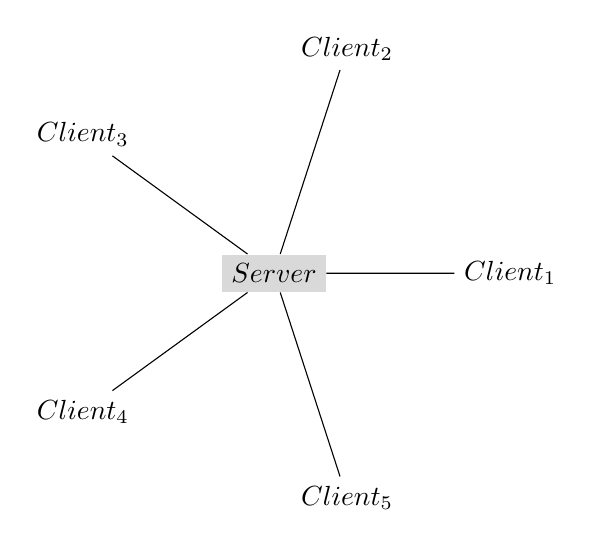
\begin{tikzpicture} [scale=1, transform shape]
%\tikzstyle{every node}=[draw,shape=circle];
\node [fill = gray!30] (v0) at (0:0) {$Server$};
\node (v1) at ( 0:3) {$Client_1$};
\node (v2) at ( 72:3) {$Client_2$};
\node (v3) at (2*72:3) {$Client_3$};
\node (v4) at (3*72:3) {$Client_4$};
\node (v5) at (4*72:3) {$Client_5$};
\draw (v0) -- (v1) % star
(v0) -- (v2)
(v0) -- (v3)
(v0) -- (v4)
(v0) -- (v5);
\end{tikzpicture}
\caption{客户\/服务器架构}
\label{CS}
\end{center}
\end{figure}

由于{\csa}的~\gss~可以验证所有~\ioc~发来的信息,所以它的防作弊能力很强。类似地,由于游戏状态永远是由~\gss~统一发布,游戏也可以很容易地达到一致性要求。正是这两个原因使{\csa}获得了许多游戏运营商的青睐。

然而,{\csa}的缺点也很多:首先,中央服务器很可能成为整个系统的性能瓶颈;其次,这类结构并不稳健,容易形成单点故障;再次,此类结构的可扩展性差,随着玩家数量的增长其服务质量将显著下降;最后,此种结构会因为不同玩家的延时差异而造成不公。

% . . . . . . . . . . . . . . . . . . . . . . . . . . . . . . . . %
\subsubsection{\pa}
% P2P架构  好处与缺点

{\pa}中每个对等体既是~\ioc~又是~\gss。没有中央服务器,每一个对等体都维护着一份游戏状态的副本。{\pa}游戏的一个著名的例子就是~MiMaze \cite{mimaze}。

{\pa}的优点很多。由于没有中央服务器,一个事件不需经过服务器验证发布的过程,可以直接发给玩家,所以它具有低延时的优点。{\pa}的另一个主要优势就是稳健性,不会因某个节点的故障而导致全局瘫痪。另外{\pa}的可扩展性很好,因为每一个加入网络的节点都会同时提供可供其他节点利用的资源。即使是大型的{\csa}也常常因为用户人数过多而导致服务器崩溃,但是{\pa}却可以达到数百万用户同时在线~\cite{real}。

\begin{figure}[htbp]
\begin{center}
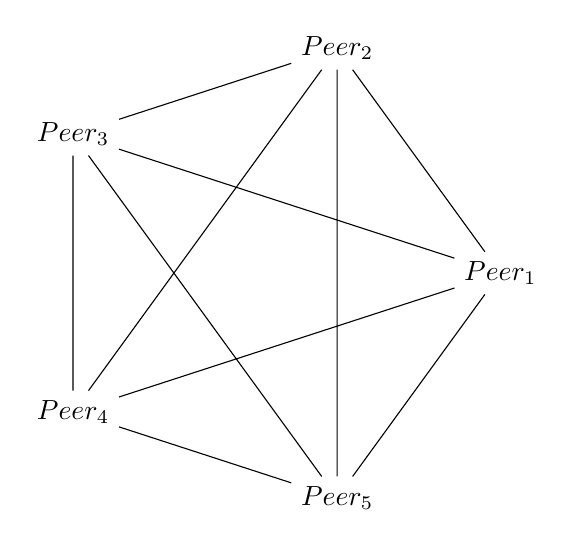
\begin{tikzpicture} [scale=1, transform shape]
%\tikzstyle{every node}=[draw,shape=circle];
\node (v1) at ( 0:3) {$Peer_1$};
\node (v2) at ( 72:3) {$Peer_2$};
\node (v3) at (2*72:3) {$Peer_3$};
\node (v4) at (3*72:3) {$Peer_4$};
\node (v5) at (4*72:3) {$Peer_5$};
\draw (v1) -- (v2) % fully connected
(v1) -- (v3)
(v1) -- (v4)
(v1) -- (v5)
(v2) -- (v3)
(v2) -- (v4)
(v2) -- (v5)
(v3) -- (v4)
(v3) -- (v5)
(v4) -- (v5);
\end{tikzpicture}
\caption{对等体架构}
\label{P2P}
\end{center}
\end{figure}


对于{\pa}网游而言,一致性的要求很可能会使可扩展性降低。比如,{\pa}常常使用全相连网络(如图~\ref{P2P}),这样每个事件产生之后就可以同时发给所有对等体,从而保证了一致性。然而,这种全相连网络的可扩展性是很差的。如果网络中有~$N$~个用户对一事件感兴趣,那么产生该事件的用户就要向网络中发出~$N$~条信息,网络中的通信量就会以玩家数量的平方数的速度增长。为了减少通信量,{\pa}常常需要依靠多播技术,然而多播技术在目前的因特网中并不普遍。幸运的是,{\pa}并不一定要使用全相连网络,许多文献中提到了用动态创建覆盖网络的方法来支持对等体间通信~\cite{p2p1, p2p2},这些方法对{\pa}的可扩展性影响较小。

另外,在{\pa}中用户认证会变得困难,收费也会变难,但是用户作弊会相对容易~\cite{cr}。

% . . . . . . . . . . . . . . . . . . . . . . . . . . . . . . . . %
\subsubsection{\da}
% 分布式架构  好处与缺点

{\da}可以看做{\csa}的进化版本。它与{\csa}类似的地方是它也拥有客户端(\ioc)和服务器(\gss)这样的分类,~\ioc~之间也不许直接连接,必须经过~\gss~中转。不过{\da}没有中央服务器,而是有分布的服务器群。游戏状态由这个群来管理。根据~\gss~组织方式的不同,{\da}又可以分为三类。

第一类:每个~\gss~维护一个游戏环节,每个~\ioc~只能连接到一个~\gss~并且只能与它交换数据。这类{\da}本质上就是多个{\csa}。它在一定程度上解决了游戏整体的可扩展性的问题,但是同时也限制了单个游戏环节的可扩展性。并且单点故障的问题仍然没有解决。

第二类:每个~\gss~维护游戏状态的一个子集。将游戏中的虚拟世界分块,每个~\gss~执掌一个块的游戏状态。~\ioc~根据其虚拟角色所在虚拟位置选择它要连接的~\gss。这样做可以显著地降低各个~\gss~的运算负担,但是同样无法解决单点故障问题。另外~\ioc~与~\gss~的连接方式会带来不公,且当虚拟角色在虚拟世界上发生大幅位移时还需要切换~\gss。

\begin{figure}[htbp]
\begin{center}
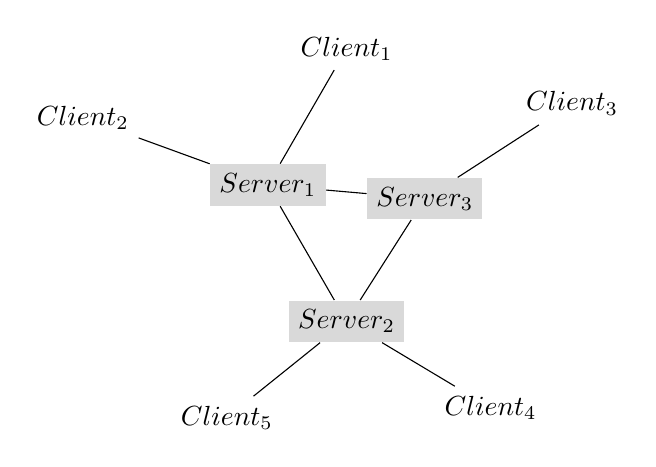
\begin{tikzpicture} [scale=1, transform shape]
%\tikzstyle{every node}=[draw];
\node [fill = gray!30] (s1) at (0:0) {$Server_1$};
\node [fill = gray!30] (s2) at (300:2) {$Server_2$};
\node [fill = gray!30] (s3) at (355:2) {$Server_3$};
\node (c1) at (60:2) {$Client_1$};
\node (c2) at (160:2.5) {$Client_2$};
\node (c3) at (15:4) {$Client_3$};
\node (c4) at (315:4) {$Client_4$};
\node (c5) at (260:3) {$Client_5$};
\draw (s1) -- (s2) -- (s3) -- (s1);
\draw (c1) -- (s1) -- (c2)
(c4) -- (s2) -- (c5)
(c3) -- (s3);
\end{tikzpicture}
\caption{\da}
\label{distributed}
\end{center}
\end{figure}

第三类:每个~\gss~维护游戏状态的一个副本。这类结构又称“{\ma}”。每个~\ioc~连接到距离它较近的~\gss,并以客户~\slash~服务器的模式与它交换数据。~\gss~之间可以用等级化的方式组织,也可以用~P2P~的方式组织(如图~\ref{distributed})。

如果使用~P2P~形式组织~\gss,那么这种结构就比较稳健,且不存在中央瓶颈。但是它也会需要一个同步机制来保障多个~\gss~之间的一致性。由于{\ma}中的~\gss~数量通常少于{\pa}中的节点数,所以{\ma}中的同步相对容易一些。





%-------------------------------------------------%
\subsection{游戏架构的八项服务}
% 网络结构需要为游戏提供的八项服务(400字)
% 见意大利论文
\label{service}

一个完整的游戏架构不应当只是由~\ioc~和~\gss~两类实体堆砌而成,而应该能够提供以下八项服务~\cite{openping, dsl}:

\begin{description}
\item[状态维护(State Maintenance)]
GSS~维护游戏状态。这个游戏状态包括虚拟世界和这个世界中所有角色的状态。

\item[一致性维持(Consistency Maintenance)]
由于不同的用户拥有不同的延时,因此他们各自看到的虚拟世界可能存在时间上的冲突和差异,因此需要提供一致性维持服务来减小甚至消除此种差异。

\item[群组管理(Group Management)]
对用户分组以及事件过滤服务也很有用,因为并非所有用户都希望得到一样的信息,这与游戏本身的语义和玩家的运算能力都有关。

\item[事件通知(Event Delivery)]
所有玩家都拥有平等的被通知权。不应该因技术原因使玩家收到通知的时间和质量存在差异。

\item[账号与认证(Accounting, Authorization)]
有时在游戏开始之初用户可以选择环境和设定参数。游戏可以通过账号来认证用户。

\item[作弊控制(Cheating Control)]
玩家的动作必须经检验才可以向其他玩家通知。一些有趣的防止作弊的方法如~\cite{cheat1, cheat2, cheat3, cheat4}。

\item[玩家间通信(Player Communication)]
玩家间实时的文字、音频、视频通信可以增强用户体验。

\item[多媒体资料传播(Multimedia Resource Distribution)]
传统观点中多媒体资料的传播仅仅局限于游戏开始之前的“离线”下载阶段~\cite{traditional}。而新兴的观点则认为多媒体资料的下载将贯穿整个游戏过程,并增强用户间互动,提升游戏的交互性~\cite{modern1, modern2, modern3}。
\end{description}


%-------------------------------------------------%

\subsection{一致性——同步的目的}
\label{def}

前文中多次提到一致性的概念。通俗地说,一致性是指:当一个事件产生时,在所有关注此事件的玩家看来这个事件都是在同一个时间发生的。更严格的一组定义如下~\cite{Ferretti2005}:

\begin{zjudefine} [安全性]
当且仅当以下条件成立时一个系统才具有安全性:在给定的时刻~$t$,所有正常工作的~\gss~所维护的游戏状态都一致,且所有故障的~\gss~都不能与正常工作的~\gss~交换数据。
\end{zjudefine}

\begin{zjudefine} [一致性]
当且仅当以下条件成立时一个系统才具有一致性:存在一条规则~$r$,当在~$r$~所规定的一系列时间检查游戏状态时,系统都能保证安全性。
\end{zjudefine}

为了达到一致性,最常用的办法是在~\gss~或对等体之间采用全序、可靠的传输,保证所有对等体或~\gss~收到的事件相同、顺序一致,从而得到一致的结果。然而现实中全序可靠的传输并不常用,因为这样的传输机制会严重影响传输性能~\cite{impact}。 因此,当下层传输协议不能提供这种服务时,就需要一个同步算法,使得各个对等体、~\gss~计算结果仿佛拥有全序可靠传输一样。

%============================%

\section{传统~IP~网络中的经典同步机制}
\label{traditional}
同步算法的目的是达到一致性(详见~\ref{def})。根据实现策略又可以分为两类:保守同步和乐观同步。保守算法致力于防止错序,即只允许~\gss~和对等体在安全的前提下处理事件。乐观算法允许错序,但是提供了检测和矫正错序的方法。~\ref{conservative}~和~\ref{optimistic}~分别介绍了经典的保守算法和乐观算法。

%-------------------------------------------------%

\subsection{保守同步算法}
\label{conservative}
保守同步算法只在安全前提下才允许~\gss~和对等体处理事件。这是通过使用本地因果限制来实现的。
\renewcommand\baselinestretch{1} %调一下脚注行间距
\footnote{相互交换信息的一组分布式进程,当且仅当它们都按照时间戳递增顺序处理事件时,称它们遵守本地因果限制。}

最有名的保守算法是~Bryant~提出的~\cite{bryant}~和~Chandy,~Misra~提出的~\cite{chandy}。这两种算法都要求进程对它将要受理的下一个事件的时间戳设置下限。高于此下限的暂时不受理,以此确保安全。为了确定这一下限,这些算法提出使用“空消息”——这是一种仅含有时间戳的消息,专门用于同步,与游戏中的其它活动都无关。但实验数据表明这些方法会严重影响系统性能~\cite{Ferretti2005}。

另一种方法是在每一个包含事件的包裹中都加入下一个尚未被处理的事件的时间戳。比如锁步算法(Lockstep synchronization)~\cite{lockstep}~就属于此类。按照此类算法,在所有成员达成一致意见以前没有一个人可以抢先处理事件,因此不一致也就不可能发生。但是这种方法无法保证游戏按照恒定的速度发展,也无法保证虚拟世界中的时间和实际时间对应,这会使在线网游的交互性大大降低,因此也不合适。

还有一种方法是固定时间桶算法(fixed time-bucket synchronization)~\cite{fixed-bucket}。这种方法通过在事件的接收方引入额外的延时来防止不一致的出现。收到的事件会先在时间桶中排队,等到规定的时间才被处理,这样就可以对收到的事件进行排序。这种方法的缺点是时间桶的大小(即最长强制等待时间)很难界定。时间桶通常取传输时间的上限,而这一上限是不明确的。时间桶取值越大,游戏的交互性就越差;时间桶取值越小,发生不一致的概率就越高。

综上所述,保守同步算法不能很好地利用并发性,对于必须以恒定速度快速快速发展的在线网游而言并不合适。
%-------------------------------------------------%

\subsection{乐观同步算法}
\label{optimistic}

最重要的乐观同步算法是{\timewarp}(Time Warp)。在这个算法中没有显式的同步行为,每个分布式进程独立按照不同速度推进游戏虚拟时间,在处理每一个事件之前先对当前游戏状态备份保存。如果收到了迟来的事件,而此事件后续的事件已经被执行了,那么游戏就回滚(rollback)至这个迟到事件之前的事件刚刚被处理完的状态。回滚包括两项任务:第一,将游戏状态恢复至迟到事件发生之前;第二,取消所有此段时间内发出的事件消息(一般使用“反消息”来取消已经发出的消息)。

{\timewarp}需要与全局虚拟时间(Global Virtual Time,简称~\gvt)配合使用。记录游戏状态需要占用大量内存,因此可以重用内存时就必须重用。~\gvt~是回滚时间戳的下限。比~\gvt~更早的状态是一致状态,不会发生回滚,因此时间戳早于~\gvt~的事件所占用的内存可以被释放。~\gvt~的定义如下:
\begin{zjudefine} [全局虚拟时间~\gvt]
一组分布式进程的待处理事件的最早时间戳。
\end{zjudefine}
% GVT的计算方法

状态跟踪算法(Trailing State Synchronization)也是一种重要的对等体同步算法。在这种算法中每个进程记录恒定数量的游戏状态(这些状态都与一个事件相关联)。游戏的状态分成两条主线发展,一条是乐观主线,所有事件都不加延时地执行;一条是延时主线,每个收到的事件都有固定延时,且在延时期间会调整错序。状态跟踪算法通过比较两条主线上的状态来检测是否有不一致发生。如果检测到不一致,则进行回滚:延时主线上的状态被拷贝到乐观主线上,并且后续事件按照正确的顺序重新执行。与{\timewarp}类似,这种算法也要在内存占有量和回滚范围之间进行权衡。

\ref{conservative}~中提到的时间桶算法还有一些乐观版本。适用于如~MiMaze~这样的简单游戏。

根据游戏具体环境和规模的不同,上述算法还存在种类繁多的衍生和变形。在此不一一赘述。


%============================%

\section{数据命名网络中的同步机制}
\label{innovative}
%(100字)

近年来出现的数据命名网络(NDN)或称内容为心网络(CCN)致力于改变传统~IP~网络上点对点的传输方式,以内容(content)作为网络的第一原语(详见外文翻译)。这一改变为网络软件的开发带来了新的机遇——网络延时的降低和网络中通信量的减少可以提升网络软件的性能。

CCN~具有继承和发展~\ref{traditional}~中所述的同步算法的潜力。CCN~的核心内容位于网络层,而同步协议位于应用层,因此前文中的游戏同步机制都可以在~CCN~中实现。与此同时,~CCN~对数据单独命名的理念和更高效的传输机制有可能推动游戏同步算法的发展,给同步协议的设计者带来启发。

CCN~网络中目前尚无游戏实例,也无专属的游戏协议。不过,~CCN~提供了一个通用的同步协议(CCNx Sync Protocol~\cite{CCNxSync}),应用程序开发员可以直接使用此协议做到数据同步(只是时间效率不高),也可以在此协议基础上开发新的协议。


\subsection{CCN~中的~SYNC~协议}
% 200字

CCN~目前提供的基础同步协议叫做~CCNx Sync\footnote{CCNx Project~是~CCN~的项目名称}。这个协议的工作前提是每个~CCN~节点都运行~CCN~仓库(CCN repository)且需要同步的节点必须直接相连。协议工作时,每个节点均有一个同步代理(Sync Agent)负责此节点与其它节点的数据一致性。每一个同步代理用一棵同步树表示和表示它所拥有的~CCN~内容,它会周期性地计算自己的同步树的哈希值,并将此值向相邻的同步代理转发。与此同时,每一个同步代理也会收到来自其它代理的哈希值。当一个同步代理将收到的哈希值与自己的哈希值比较,发现有出入时,它会发出一个~CCN Interest~包,以获取造成这种差异的同步树中的节点的名字。这个~Interest~包会得到一个~CCN Data~包的回复,这样该同步代理就拥有了它所缺失的数据的名字。在此之后,该代理会发出新的~Interest~去获取它所缺失的数据。当所有缺失的数据都到达时,此同步代理重新计算出的同步树的哈希值就会与它邻接代理的值一致。换言之,此同步代理与它的邻接代理之间的同步工作就暂时完成了。

CCNx Sync~协议的优点在于它以同步树的方式同步数据。这意味着使用此协议的软件可以灵活地将同步工作区分成很多子任务,不但减少了同步算法的工作量,而且可以去除不必要的延时等待。此协议的缺点是所有需要同步的数据都必须先写入本地的~CCN~仓库才可以进行同步,导致同步的速度过慢,不适合运用于时间要求很高的同步。另一个缺点是所有的同步节点都要运行~CCNx Sync~协议,且要直接相连,这给网络的可扩展性带来很大限制。最后,~CCN~仓库目前尚不支持内容删除,这意味着软件运行一定时间后必须关闭以清空仓库中的大量过期内容。

CCNx Sync~协议与前文中的游戏同步协议是有区别的。CCNx Sync~侧重于维持数据一致性,而游戏同步协议则在数据一致的情况下还需要保证数据按照正确的顺序被处理。因此,如果需要在~CCN~网络中实现游戏同步,还需要开发人员选择或设计新的同步协议。


%============================%

\section{结论}

大型多人网络游戏(MMOG)是一类重要的网络应用软件,其游戏架构可以分为{\csa}、{\pa}和{\da}。其中后两者因为可扩展性强、延时小、无单点故障等原因在学术界收到广泛重视。游戏同步算法是{\pa}和{\da}必须使用的算法。它可以分为保守和乐观两大类。乐观类同步算法不需强制使用延时,与保守类算法相比时间性能较好,对游戏交互性影响较小。

随着新兴的数据命名网络(NDN)的发展,网络主机之间的通信方式被改变,网络中的同步协议将在~NDN~中得到继承,并有可能获得新的发展空间。由于~NDN~和其它新兴网络架构目前尚处于研发阶段,这些网络架构目前在网络游戏以及游戏同步方面的协议实现和协议设计尚属空白。

\bibliography{data/zjubib}






